% Figure captions for the inertia-elbow plots.

\begin{figure*}
\centering
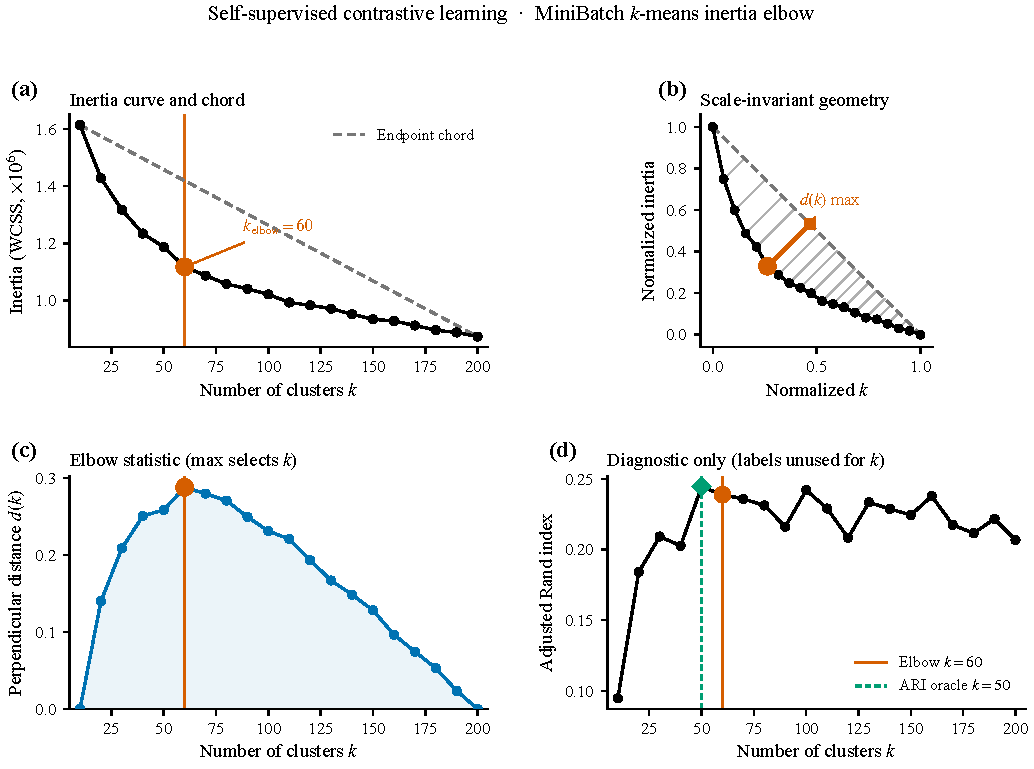
\includegraphics[width=\textwidth]{figures/fig_elbow_method}
\caption{\label{fig:elbow_method}
Unsupervised selection of $k$ by the MiniBatch $k$-means inertia elbow
(self-supervised contrastive embeddings; $184{,}603$ frames).
The $k$-sweep recorded several scores, but only inertia (WCSS) was used
to choose $k$.
(a)~Inertia versus $k=10,20,\ldots,200$, with the endpoint chord (dashed).
(b)~The same curve after min--max normalizing both axes; gray segments are
perpendiculars to the chord and the orange segment is the longest.
(c)~That distance $d(k)$. The maximizer is $k=60$.
(d)~ARI versus $k$, diagnostic only: labels were not used to choose $k$.}
\end{figure*}

\begin{figure*}
\centering
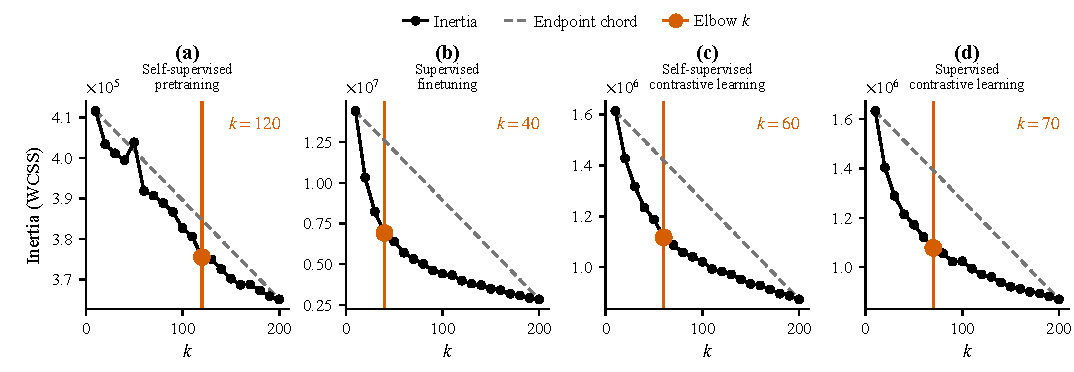
\includegraphics[width=\textwidth]{figures/fig_elbow_four_models}
\caption{\label{fig:elbow_four_models}
Inertia versus number of clusters $k$ for the four representations
in Sec.~\ref{sec:compared_reps}
(training split, $184{,}603$ frames).
(a)~Self-supervised pretraining, elbow $k=120$.
(b)~Supervised finetuning, $k=40$.
(c)~Self-supervised contrastive learning, $k=60$.
(d)~Supervised contrastive learning, $k=70$ (seed 42, 50-50 noise coin).
The dashed line is the endpoint chord; the orange mark is the inertia elbow.}
\end{figure*}

\begin{figure*}
\centering
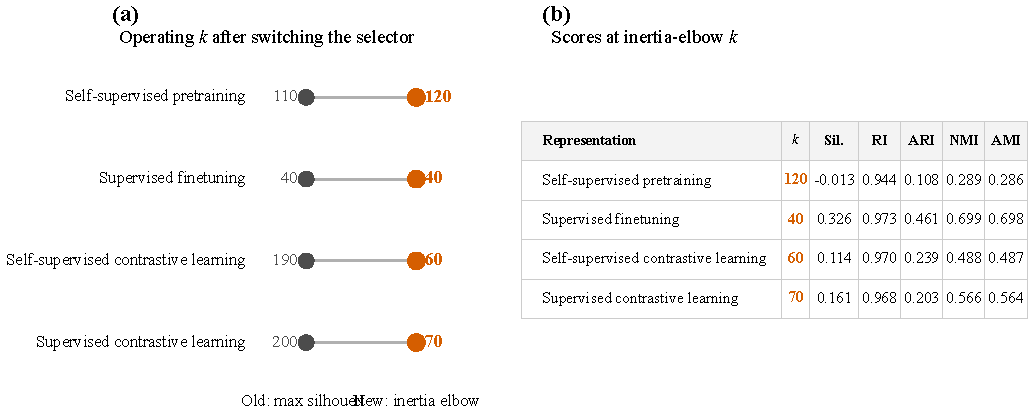
\includegraphics[width=\textwidth]{figures/fig_elbow_operating_points}
\caption{\label{fig:elbow_operating_points}
Latest evaluation uses the inertia elbow, not max silhouette.
(a)~Change in operating $k$ when the selector is switched.
(b)~Clustering scores at the inertia-elbow $k$ on the training split.}
\end{figure*}
